% !Mode:: "TeX:UTF-8"

\chapter{使用kmeasn++算法结合位翻转算法进一步提高压缩率}

测试立方压缩旨在通过提高压缩率,降低测试时间、节约压缩成本。测试立方由一系列0、1以及无关位$X$组成,其中$X$ 既可以被填充为0 也可以被填充为1,而不影响原测试集的故障覆盖率,因此包含较多无关位的测试集往往会获得较高的压缩率。本章将使用位翻转算法在不影响故障覆盖率的前提下,通过增加原测试集的无关位提高压缩率。

\section{相关概念}

\subsection{故障检测冗余度}
故障检测冗余度通俗的来说就是同一个故障在测试过程中被多次检测。比如,数据冗余是指某个数据在特定情况下反复出现,那么故障检测冗余度类也是类似的。测试集由ATPG产生,初始测试集中包含大量数据,其中存在众多的无关位。由于可以将部分无关位会被转化成为确定位,测试集的规模会大大减小,但测试立方整体的故障覆盖率保持不变。

\subsection{位翻转}
本文主使用拆分压缩的方式提高压缩率,拆分压缩会将原测试立方拆分成为主分量集和残分量集,如果主分量集和原测试集高度相似便会提高残分量集的压缩率。假设主分量的故障覆盖率为$A$,测试立方的总故障覆盖率为$C$,剩余故障覆盖率为$C-A$。通过故障模拟之后原测试立方只要能检测出剩余故障即可,为了避免相同故障被反复检测可以将原测试立方中特定的确定位翻转为$X$,在总故障覆盖率不变的情况下,提高压缩率。这个过程被称之为位翻转。

\subsection{位翻转应用于压缩}
原测试集中包含的确定位会影响最终的压缩率,如果可以将部分确定位翻转成为无关位,将无关位按照有利于压缩的方向填充便能提高压缩率。为了降低硬件开销以及实验复杂度本人使用的是一轮位翻转,具体过程分为下述几个步骤:1、结合第三章与第四章的算法将原测试拆分成为主分量集和残差集。2、将主分量集进行故障模拟,记录能检测的故障数$A$,在不影响故障覆盖率的前提下将原测试集中的某些确定位翻转成为无关位$X$,生成新的测试集。3、将新的测试中的无关位进行填充然后与原主分量集进行异或,在本实验中无关位的填充方式主要根据主分量集对应的位进行填充。

下图\ref{51}为位翻转应结合本实验的压缩过程:图中可以看出原测试立方的故障覆盖率达100\%,拆分压缩之后的主分量集能取得的故障覆盖率可达到70\%,剩余故障为30\%。在保证故障覆盖率的条件下,将原测试集部分确定位翻转为无关位并获得新测试集,根据主分量的确定位对原测试集的无关位进行填充,最后将主分量集与已填充的测试集进行异或得到最终需要进行压缩的新残差集。

\begin{figure}[H]
  \centering
  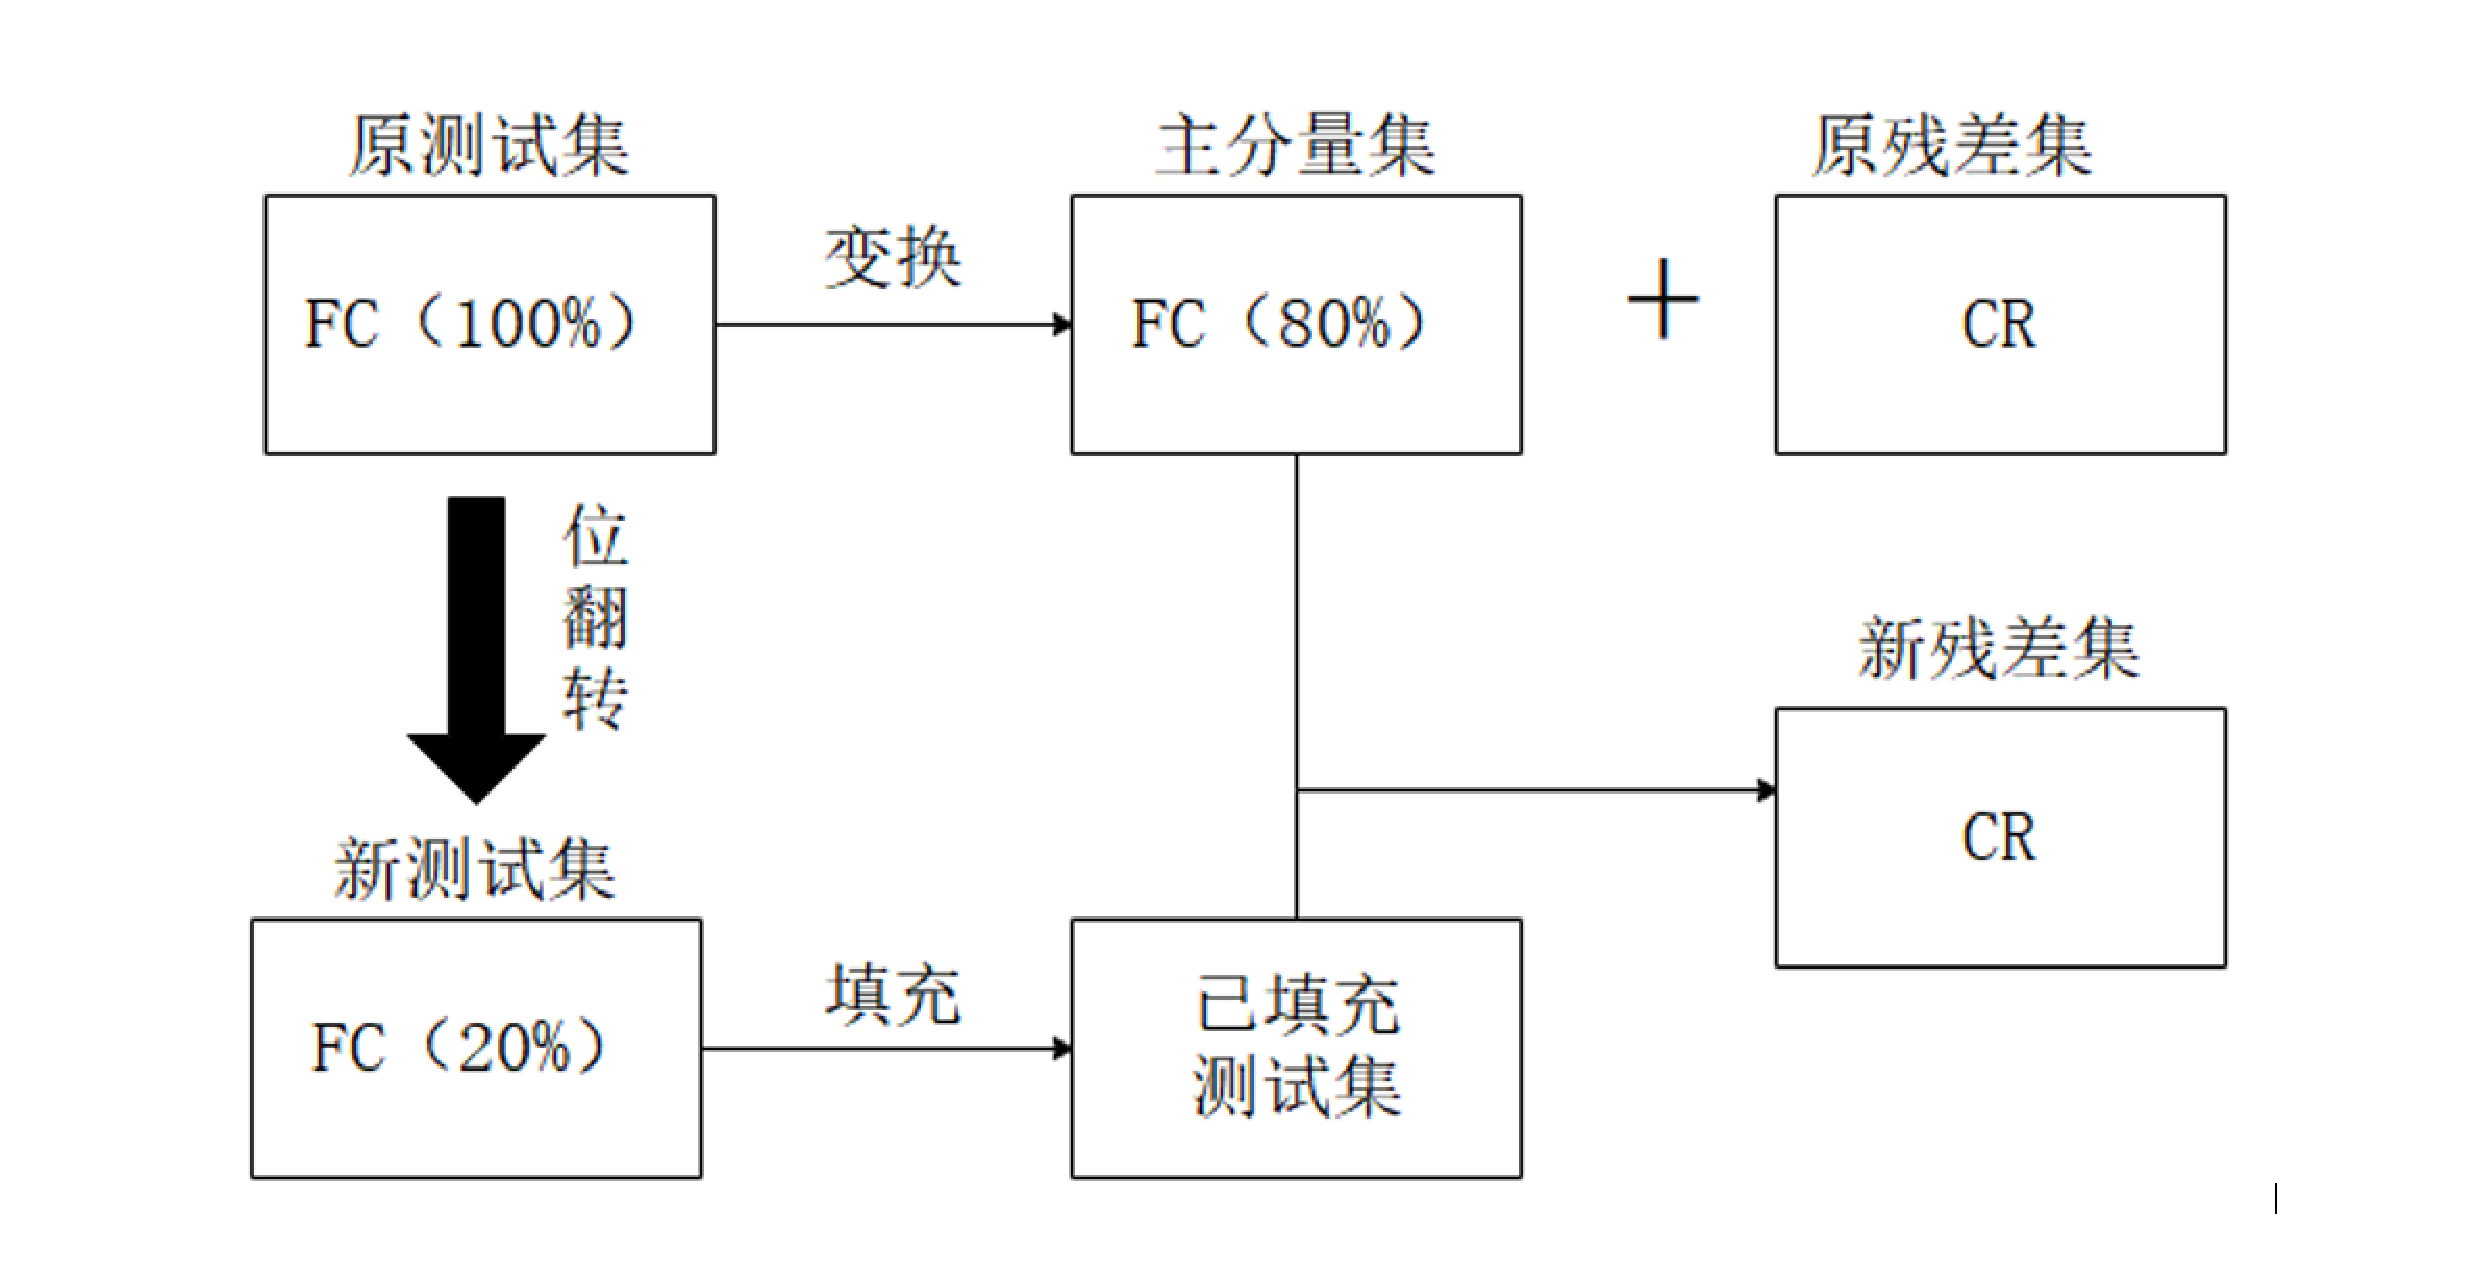
\includegraphics[height=8cm,width=16cm,angle=0,scale=1]{51.eps}
  \caption{FDR编码方式折线图}\label{51}
     \end{figure}

在论文“多次随机变换拆分测试激励压缩方法研究”\cite{76}中提及了多轮位翻转算法,但是由于每一轮翻转,均会产生代价,并且硬件代价与实现相对比较困难,本人化繁为简直接使用一轮压缩,然后根据主分量集对原测试集进行二次填充,在保证压缩率的前提下节约了硬件开销以及存储代价。

\section{翻转算法}
若$C$代表原测试集合的故障覆盖率,对原测试集进行位填充之后,拆分为主分量集和残差集,$A$代表主分量集合所能达到的故障覆盖率,假设原测试集合的故障覆盖率$B$,只需要满足$B>C-A$即可,下文将基于这种思路写出位翻转算法的伪代码。

\begin{algorithm}[!h]
	\caption{位翻转基本过程}%算法标题
	\begin{algorithmic}%一行一个标行号
        \STATE $CoverageC$  //原测试集的故障覆盖率
		\STATE $CoverageA$ $ $//拆分原测试集后主分量集的故障覆盖率
        \STATE $CoverageC$  $ \leftarrow $  $FaultCoverage$ $(T)$
        \STATE $CoverageB$  $ \leftarrow $  $FaultCoverage$ $(L)$
		\FOR{$bit$ in $T$}
        \IF{$bit$ = $1$ or $0$}
		\STATE $bit$  $ \leftarrow $  $X$
		\ENDIF
        \IF{$Coverage$ $<$ $CoverageA$ $-$ $CoverageB$}
		\STATE $bit$  $ \leftarrow $  $1$ $or$ $0$
		\ENDIF
		\ENDFOR
        \STATE $Return$ $T$
	\end{algorithmic}
\end{algorithm}

算法5.1为翻转测试集的基本过程,首先将原测试立方中的确定位一一翻转,并进行故障模拟,如果不影响故障覆盖率则直接翻转,反之还原,若故障模拟的时间为$t$,翻转一位的时间为$s$,假设原测试集合中由$k$个确定位,那么算法的时间复杂度为$kts$,理论上而言该算法可以通过较小的代价取得较高的压缩率。

\section{实验结果与分析}
为了说明kmeans++算法结合位翻转算法确实有效,本文对S5378、S9234、S13207、S15850等电路进行了实验。本章将挑选其中部分电路做具体描述,本文选取选取了FDR、EFDR、ALT-FDR编码方式对变换拆分之后的残差集进行压缩,同时与直接使用位翻转算法所达到的压缩率进行对比。

实验结果如下所示,表\ref{btabl1}-\ref{btabl3}分别表示各方法在FDR、EFDR、 ALT-FDR编码下缩能达到的压缩率,其中第一列为电路名称,第二列表示对测试集直接编码所能取得的压缩率,第三列表示使用原测试集集合kmeans++算法所能达到的压缩率,第四列表示对测试集直接翻转所达到的压缩率,第五列为使用本方法所达到的压缩率。

\begin{table}[H]
\centering
\caption{FDR编码压缩率(\%)}\label{btabl1}
\begin{tabular}{p{2.2cm}p{2.7cm}<{\centering}p{3.3cm}<{\centering}p{2.7cm}<{\centering}p{2.7cm}<{\centering}}
\toprule
\textbf{电路}&	\textbf{直接编码}& \textbf{Kmeans++聚类}& \textbf{直接翻转}& \textbf{本方法}\\
\midrule
s5378&	47.98&	70.76&	78.06&	79.69\\
s9234&	43.61&	69.59&	74.01&	78.06\\
s13207&	81.31&	92.29&	91.93&	94.93\\
s15850&	66.21&	81.75&	86.04&	86.27\\
s38417&	43.21&	75.35&	78.71&	80.31\\
平均&	56.46&	77.95&	81.75&	83.85\\
\bottomrule
\end{tabular}
\end{table}

\begin{table}[H]
\centering
\caption{EFDR编码压缩率(\%)}\label{btabl2}
\begin{tabular}{p{2.2cm}p{2.7cm}<{\centering}p{3.3cm}<{\centering}p{2.7cm}<{\centering}p{2.7cm}<{\centering}}
\toprule
\textbf{电路}&	\textbf{直接编码}& \textbf{Kmenas++聚类}& \textbf{直接翻转}& \textbf{本方法}\\
\midrule
s5378&	53.67&	67.75&	76.16&	77.68\\
s9234&	48.66&	66.14&	71.28&	75.85\\
s13207&	82.49&	91.60&	91.53&	94.52\\
s15850&	68.66&	79.84&	84.24&	84.99\\
s38417&	62.02&	74.06&	78.24&	79.13\\
平均&	63.0&	75.88&	80.29&	82.43\\
\bottomrule
\end{tabular}
\end{table}

\begin{table}[H]
\centering
\caption{ALT-FDR编码压缩率(\%)}\label{btabl3}
\begin{tabular}{p{2.2cm}p{2.7cm}<{\centering}p{3.3cm}<{\centering}p{2.7cm}<{\centering}p{2.7cm}<{\centering}}
\toprule
\textbf{电路}&	\textbf{直接编码}& \textbf{Kmenas++聚类}& \textbf{直接翻转}& \textbf{本方法}\\
\midrule
s5378&	49.95&	65.17&	72.17&	76.26\\
s9234&	45.14&	62.72&	67.61&	73.50\\
s13207&	80.12&	90.88&	88.93&	94.09\\
s15850&	65.64&	77.82&	81.64&	83.85\\
s38417&	60.52&	71.23&	75.32&	76.93\\
平均&	60.27&	73.56&	77.13&	80.93\\
\bottomrule
\end{tabular}
\end{table}

从上表可以看出本方法能极大地提升残差集的压缩率,比对电路直接编码所达到的平均压缩率高22.49\%,比对原测试集直接翻转所取得的平均压缩率高2.68\%。

\section{小结}
位翻转方法旨在通过将确定位翻转为无关位来提高压缩率。由于主分量集自身可以检测出部分故障,原测试集只需检测剩余故障即可。通过故障模拟,原测试将某些确定位翻转为无关位后,得到了一个新测试集,新测试集填充无关位之后与主分量异或得到了新的残差集,此时的残差集包含的0比特位大大增加,能进一步提高压缩率。使用kmeans++算法集合位翻转的压缩方法,能使压缩率在第四章的基础上提高7\%。


